\documentclass[conference]{IEEEtran}
\IEEEoverridecommandlockouts
\usepackage[T1]{fontenc}
\usepackage{amsmath,amssymb,amsfonts}
\usepackage{algorithm}
\usepackage{algpseudocode}
\usepackage{graphicx}
\usepackage{booktabs}
\usepackage{multirow}
\usepackage{xcolor}
\usepackage{url}
\usepackage{tikz}
\usetikzlibrary{arrows.meta,positioning,fit}
\usepackage[hidelinks]{hyperref}
\usepackage{cite}
% Visible placeholder for any number that is not yet backed by a completed run.
\newcommand{\TBD}[1]{\textcolor{red}{\textbf{[TBD: #1]}}}

\begin{document}

\title{CARMA: Candidate-based Attribution of Root\\ Failures in LLM Multi-Agent Systems}

\author{\IEEEauthorblockN{Muhammad Umar Farooq}
\IEEEauthorblockA{\textit{Department of Computer Science}\\
\textit{National University of Computer and Emerging Sciences (FAST-NUCES)}\\
Islamabad, Pakistan\\
i267832@isb.nu.edu.pk (corresponding author)}}

\maketitle

\begin{abstract}
When a multi-agent system built on large language models fails, the step that exposes the failure is often not the step that caused it, and published attribution results are hard to compare because evaluation conditions differ. We reproduce the All-at-Once judge of the Who\&When benchmark under a fixed protocol with strict scoring (52.4\% agent and 14.3\% step accuracy, within two points of the published values) and find that on unnumbered logs it never predicts step~0, where 20 of 126 decisive errors lie. We propose CARMA: Dense Candidate Scoring (DCS) asks the judge, in one call, for a scored list of candidate error steps over a numbered log, and Cascade-Aware Root Resolution (CARR) re-ranks the list with a deterministic artifact-provenance graph. We also build CARMA-Cascade, which adds one injected later error to each log. With two open-weight judges, DCS raises step accuracy by 26--28 points over the official protocol ($p<0.001$), but controls show that numbering the log alone gives 16.7 of these points for the stronger judge, against which DCS's remaining gain is not significant ($+9.5$, $p=0.065$; weaker judge $+19.0$, $p<0.001$). The clearest benefit of the DCS prompt is resistance to distraction: on CARMA-Cascade, numbered All-at-Once picks the injected step in 45.9\% and 33.3\% of logs, DCS in 5.4\% and 14.4\% (both $p<0.001$). The candidate list contains the decisive step in 85\% of logs and serves as a rollback schedule. CARR never changes the stronger judge's prediction, because its probabilities are strongly over-confident (calibration error 0.38). Code, data and results: \url{https://github.com/umarfarooq478/traid-mas}
\end{abstract}

\begin{IEEEkeywords}
failure attribution, multi-agent systems, large language models, LLM-as-a-judge, error propagation
\end{IEEEkeywords}

\section{Introduction}
Large language models (LLMs) are now deployed as \emph{agents}: they reason over many turns, call external tools such as code interpreters and web browsers, and act on what those tools return~\cite{yao2023react,shinn2023reflexion}. A single agent on a long task soon runs into limits. Its context fills up, one prompt has to cover planning, coding and checking at once, and nothing independent checks its output. The usual response is to split the work across several specialised agents that talk to each other through a shared conversation. A planner breaks the task down, a coder writes and runs code, a verifier checks the result. Frameworks such as AutoGen~\cite{wu2024autogen}, MetaGPT~\cite{hong2024metagpt} and CAMEL~\cite{li2023camel}, and multi-agent debate~\cite{du2024debate}, are built this way, and they are evaluated on demanding benchmarks such as SWE-bench~\cite{jimenez2024swebench} and GAIA~\cite{mialon2024gaia}.

These systems fail often. An analysis of more than 1,600 annotated traces from seven multi-agent frameworks found that the gains over single-agent baselines are often small, and that failures fall into recurring modes of system design, inter-agent misalignment and missing verification~\cite{cemri2025why}. Many of these modes come from how the agents are organised, not from the underlying model, so a stronger model alone does not remove them. Topology matters as well. When one agent is made faulty, hierarchical teams lose 5--12\% of their performance and linear chains up to 24\%~\cite{huang2025resilience}, and the interaction structure changes how vulnerable a system is to adversarial agents~\cite{kavathekar2026tamas}.

Failures in these systems are also hard to trace. Each agent conditions on what the others wrote, so an early mistake travels through later messages, and none of those messages looks wrong on its own. The mistake might be a misread instruction, a wrong argument passed to a tool, or an intermediate number that nobody checked. When the final answer finally comes out wrong, the step that shows the failure is usually not the step that caused it. \emph{Failure attribution} is the task of finding the cause: given a failed run, name the agent and the step that were decisively responsible~\cite{zhang2025whowhen}. It differs from failure classification, which assigns a failure \emph{type} to a run, because it must point to one place in one execution. Debugging needs that answer, and so does any mechanism that rolls a run back to fix it~\cite{ma2025dover,feng2026conformal}. Done by hand it means reading entire traces: building the first benchmark, Who\&When, took each annotator tens of hours~\cite{zhang2025whowhen}.

The founding work defined the task as recovering one decisive (agent, step) pair and tested three ways of asking an LLM to act as the judge~\cite{zhang2025whowhen}. \emph{All-at-Once} shows the judge the whole log and asks for the agent and step in one answer. \emph{Step-by-Step} walks through the log and asks, after each step, whether this is the decisive error. \emph{Binary Search} asks which half of the log contains the error and recurses. Over the whole benchmark, the best of them reached 53.5\% accuracy on the agent but only 14.2\% on the step. On the algorithm-generated subset with GPT-4o, Step-by-Step was best at the step level with 25.5\%, and All-at-Once, at 12.5\%, was below a random baseline (19.1\%). Finding \emph{when} a failure happened is much harder than finding \emph{who} caused it.

Work since then has gone in four directions. The first keeps the LLM judge and restructures its reasoning: RAFFLES iterates between a reasoner and specialised evaluators until a decisive fault is agreed~\cite{zhu2026raffles}, and A2P scaffolds abduction, intervention and outcome prediction in the judge's prompt~\cite{west2025a2p}. The second trains a dedicated model. AgenTracer creates labelled failures by counterfactual replay and fault injection and trains an 8B tracer that beats much larger judges~\cite{zhang2026agentracer}. The third borrows from software testing. FAMAS replays a failing task many times and scores each action by how much more often it appears in failing runs than in successful ones~\cite{ge2026spectrum,wong2016survey}. The fourth builds a dependency or causal graph over the trace, with extra LLM calls, search or reinforcement learning, so that a root cause can be told apart from the symptoms it produced~\cite{zhang2025graphtracer,wang2026chief,rafi2026falat,ma2025causal}. In parallel, runtime systems such as MASC, EAGER and LumiMAS try to catch a bad step while the run is still going and trigger a correction before the error spreads~\cite{shen2026masc,zhang2026eager,solomon2026lumimas}.

Despite this activity, it is hard to say whether the field is improving, and three gaps stand out.

\textbf{(G1) Reported numbers are hard to compare.} Methods are evaluated under different conditions, and the conditions matter a great deal. Showing the judge full execution traces instead of agent outputs alone raises attribution accuracy by up to 76\% (relative) on the same failures~\cite{chen2026elephant}. Prefixing every message with its step index raises a causal judge's step accuracy from 17.8\% to 47.5\%~\cite{west2025a2p}. And the official scoring script of~\cite{zhang2025whowhen} accepts a predicted step whenever the gold index is a \emph{substring} of it, so a gold step ``1'' matches a prediction of ``12''. A reported gain therefore cannot be credited to a method unless formatting, observability and scoring are held fixed.

\textbf{(G2) The single-step formulation has not been tested on cascading errors.} Every method above returns one step. Real traces can contain several faulty messages, and a judge looking for one step may be drawn to a later, more visible error instead of the earlier one that decided the outcome. No study we reviewed measures this \emph{distraction} directly.

\textbf{(G3) Attribution is not connected to recovery.} The runtime systems use cheap detectors and report detection quality and task success. The attribution methods report localisation accuracy and are never used to trigger a correction. Whether a predicted step would be a good point to roll back to, and at what cost, is rarely measured~\cite{feng2026conformal,shen2026masc,zhang2026eager}.

We address these gaps with three objectives. \textbf{O1}: re-implement the judges of~\cite{zhang2025whowhen} and evaluate every method under one fixed protocol (fixed observability, fixed access to the correct answer, strict scoring), with controls that separate log formatting from the method itself. \textbf{O2}: build trajectories that contain a second, later error and test whether an attribution method stays on the decisive step, without training or extra LLM calls. \textbf{O3}: score each predicted step, and each ranked list of steps, as a rollback trigger, including how much correct work it would throw away and what it costs.

We call the resulting framework CARMA (Candidate-based Attribution of Root failures in Multi-Agent systems). It has a method part and an evaluation part. The method, Dense Candidate Scoring (DCS), asks the judge once for a short scored list of suspect steps over an explicitly numbered log, with a prompt that defines the decisive error and warns that later steps may only expose it. A deterministic re-ranker, Cascade-Aware Root Resolution (CARR), then uses a graph of which earlier step first produced each artifact that later steps reuse. The evaluation part is a controlled protocol and CARMA-Cascade, a version of Who\&When with one injected later error per log.

The results are more modest than a first comparison suggests, and more informative. DCS raises strict step accuracy over the official All-at-Once protocol by 26--28 points with two open-weight judges. But adding step numbers to All-at-Once alone gives 16.7 of those points with the stronger judge, and against that numbered baseline the remaining gain is not significant for that judge. Where DCS clearly helps is distraction. With one injected later error, numbered All-at-Once moves to the injected step in 33--46\% of logs, DCS in 5--14\%. The contributions are:
\begin{enumerate}
\item \textbf{A controlled evaluation protocol and reproduction.} Strict scoring, fixed observability and ground-truth settings, tolerance and top-$k$ accuracy, trivial reference baselines, rollback metrics, cost accounting, paired bootstrap intervals, exact McNemar tests and a run-to-run drift check. Applied to the base paper, it reproduces All-at-Once within two points and shows that, on unnumbered logs, the judge never predicts step~0 and, in about three quarters of logs, names an agent who did not speak at the step it predicted.
\item \textbf{Dense Candidate Scoring (DCS)}, a one-call attribution method that returns a scored list of candidate steps over a numbered log. It raises strict step accuracy by 26--28 points over the reproduced baseline. Controls that add step numbers to All-at-Once and restrict DCS to one candidate show that numbering accounts for most of the gain with the stronger judge, whose DCS is not significantly better than numbered All-at-Once ($+9.5$ points, $p=0.065$). The prompt's further gain is partly a bias towards early steps, and the list does not improve the first answer but is a useful ranking (Table~\ref{tab:decomp}).
\item \textbf{CARMA-Cascade}, a multi-error version of Who\&When made by injecting one extra, independent error after the annotated decisive step, written by a different LLM from the judge. It comes with a distraction rate, its pre-injection and chance levels, and a manipulation check. On it, numbered All-at-Once is drawn to the injected step in 33--46\% of logs and DCS in 5--14\%, which separates the effect of the DCS prompt from that of numbering.
\item \textbf{An analysed negative result.} CARR never changes the main judge's prediction. The reason is that DCS probabilities rank well but are strongly over-confident, so a bounded multiplicative correction cannot overturn them, even though a perfect re-ranker of the same lists could reach 84.9\% (the share of logs whose gold step is in the DCS list).
\end{enumerate}

Section~\ref{sec:related} reviews related work. Section~\ref{sec:method} describes the data, the problem formulation and the method. Section~\ref{sec:exp} reports the setup, the reproduction, the results and the ablations, and Section~\ref{sec:concl} concludes.\footnote{This work extends an earlier, purely evaluative course proposal by adding DCS and CARR as concrete mechanisms, turning its research questions into measurable experiments, and limiting the intervention objective to an offline rollback analysis that can be computed on the public benchmark.}

\section{Related Work}\label{sec:related}
We group prior work by how attribution evidence is obtained (prompting, training, replay or graphs) and by when it is used (after the run or during it). The disagreements in this literature are mostly methodological, so this grouping shows more than a chronological one.

\subsection{Why multi-agent systems fail}
Cemri et al.~\cite{cemri2025why} analysed more than 1,600 traces from seven frameworks and derived a taxonomy of 14 failure modes in three categories: system design, inter-agent misalignment, and task verification. Annotators agreed well on these modes ($\kappa=0.88$), and design failures dominated. The taxonomy says what \emph{kind} of failure a run shows, across a population of runs. It does not say which agent or step in a given run was responsible, which is the question attribution asks. Two studies show that structure is a reliability variable in its own right. Huang et al.~\cite{huang2025resilience} injected faults into agents' messages or profiles (AutoInject, AutoTransform) and found that hierarchical teams are far more resilient than linear chains, and that adding a challenger and an inspector role recovers up to 96.4\% of the lost performance. TAMAS~\cite{kavathekar2026tamas} benchmarks multi-agent systems against 300 adversarial instances of six attack types and finds that the interaction configuration changes how vulnerable a system is. Both improve robustness without diagnosing anything, which leaves open how much an accurate attribution adds on top.

\subsection{Prompted LLM judges}
Zhang et al.~\cite{zhang2025whowhen} defined automated failure attribution and released Who\&When: 184 failed trajectories from 127 multi-agent systems on GAIA~\cite{mialon2024gaia} and AssistantBench~\cite{yoran2024assistantbench}, each annotated with a responsible agent, a decisive step and a rationale. Their three judges trade context for focus. All-at-Once (AAO) reads the whole log and is best at naming the agent. Step-by-Step (SBS) judges one step at a time and is best at the step, at the cost of up to $T$ calls for a log of $T$ steps. Binary Search (BS) halves the log recursively. All three inherit the known biases of LLM judges~\cite{zheng2023judging} and degrade on long contexts~\cite{liu2024lost}. The formulation is deliberately minimal, which made it easy to adopt, but it builds in two assumptions that later work kept: exactly one decisive step per trajectory, and a judge that sees only the agents' messages. RAFFLES~\cite{zhu2026raffles} keeps the judge but restructures its reasoning. A reasoner proposes candidate faults, specialised evaluators test them against explicit decisiveness criteria, and the loop repeats until a decisive fault is agreed. This helps on long traces where single-pass judging fails, but it pays for repeated full-context reasoning and is designed as an offline tool.

\subsection{Learned and statistical attribution}
AgenTracer~\cite{zhang2026agentracer} addresses the shortage of step-level labels by generating them. It takes successful runs, corrupts them by counterfactual replay and programmed fault injection, and trains a compact 8B tracer with reinforcement learning on the result; the tracer outperforms much larger proprietary judges, which suggests that attribution is better learned than prompted. Its faults, however, are single and independent by construction, and whether they resemble naturally occurring ones is not tested. FAMAS~\cite{ge2026spectrum} adapts spectrum-based fault localisation from software testing~\cite{wong2016survey}. It replays a failing task many times and scores each action by how disproportionately it appears in failing runs. It needs neither labels nor a trained model, and its suspiciousness scores are computed rather than asserted by a model that may hallucinate. In exchange it needs runs that can be repeated without side effects and that vary enough between replays, which holds for benchmark tasks but not for agents that write files, call paid APIs or change live state.

\subsection{Causal and dependency-aware attribution}
A closely related line tries to separate root causes from the symptoms they produce. A2P~\cite{west2025a2p} scaffolds three stages in the judge's reasoning: abduction (what went wrong), action (what correction to apply) and prediction (whether the run would then succeed). It reports 47.46\% step accuracy on the algorithm-generated and 29.31\% on the hand-crafted subset of Who\&When. Its ablation matters for this paper: removing the ``Step $t$ -'' prefixes from the log lowers its algorithm-generated step accuracy to 17.78\%, so most of its gain over its own 16.67\% All-at-Once baseline comes from numbering. Ma et al.~\cite{ma2025causal} apply causal inference at several granularities. GraphTracer~\cite{zhang2025graphtracer} builds information-dependency graphs and trains a tracer with graph-structural rewards. CHIEF~\cite{wang2026chief} turns logs into a hierarchical causal graph and screens candidates counterfactually. FALAT~\cite{rafi2026falat} searches over typed dependencies and checks whether correcting a candidate would recover the outcome. Together these show that dependency structure matters, but they obtain it with extra LLM calls, training or replay, and they are evaluated against single-decisive-step labels.

\subsection{Observability, uncertainty and evaluation}
Seeing the Whole Elephant~\cite{chen2026elephant} argues that attribution must be studied under full observability. Existing benchmarks record agents' outputs but omit the inputs, system prompts, tool logs and configuration that a developer looks at when debugging. The authors build a benchmark of 220 failed traces with reproducible environments and re-evaluate existing methods under matched conditions. Full traces raise accuracy by up to 76\% relative to partial ones; on identical failures, step accuracy rises from about 16\% to 28--30\% and agent accuracy from 51\% to 62\%. Two consequences follow. Part of the reported difficulty of step-level attribution is an artefact of what was recorded, and accuracies from papers with different observability cannot be compared. The same study reports only moderate inter-annotator agreement on step labels ($\kappa=0.64$), which qualifies the single-decisive-step ground truth that all methods optimise. Two other works treat attribution as uncertain. Conformal Agent Error Attribution~\cite{feng2026conformal} replaces a point prediction with a contiguous set of steps that carries a coverage guarantee, and uses it for rollback. DoVer~\cite{ma2025dover} treats each attribution as a hypothesis to be tested by intervening on the run, notes that Who\&When labels are themselves uncertain, and reports that judges hallucinate step indices unless the log is numbered.

\subsection{Runtime detection and intervention}
A parallel family acts during execution, where latency and label-free operation matter more than precise localisation. AGDebugger~\cite{epperson2025interactive} lets a developer inspect, edit, reset and steer messages in a running system; it showed that mid-run intervention is feasible but left every decision to a person. MASC~\cite{shen2026masc} automates detection. It predicts the next step's representation from the interaction history, flags a step whose actual content deviates, and hands it to a correction agent before the error spreads; it reports up to 8.47\% higher detection AUC (area under the ROC curve) and consistent end-to-end gains. EAGER~\cite{zhang2026eager} learns contrastive representations of reasoning traces for real-time detection and mitigation, motivated explicitly by the cost of per-trace LLM reasoning. LumiMAS~\cite{solomon2026lumimas} layers lightweight anomaly detectors under an explanation stage that runs root-cause analysis only when needed. These systems share a design choice: each picks a detector that is cheaper and less precise than the attribution methods above and justifies it by efficiency. Each also reports detection or task metrics rather than decisive-step accuracy, so whether the cheaper detector gives up much recovery has not been tested.

\subsection{Positioning}
Table~\ref{tab:related} summarises the comparison. Papers report accuracy under different observability, formatting, ground-truth and scoring conventions, so their rankings cannot be compared directly (G1). Every method is trained or evaluated against one decisive step, and none measures how often a later error pulls it away from that step (G2). The dependency-aware methods that could separate roots from symptoms pay for their graphs with extra calls, replay or training, which is the cost runtime systems avoid, and few studies score an attribution as a rollback trigger (G3). CARMA stays within one LLM call per log, uses message-level injection in the spirit of AutoInject~\cite{huang2025resilience} to test attribution rather than task success, and treats numbering as a controlled variable rather than as part of the method.

\begin{table*}[t]
\centering
\caption{Comparison of the most relevant attribution approaches. ``Calls'' is the number of LLM calls per trajectory at inference ($T$ = number of steps). Step accuracies are on the algorithm-generated Who\&When subset with ground truth, as reported by each paper (different backbones; not directly comparable).}
\label{tab:related}
\footnotesize
\setlength{\tabcolsep}{3pt}
\begin{tabular}{@{}p{2.2cm}p{3.6cm}p{2.3cm}p{1.6cm}p{3.3cm}p{3.6cm}@{}}
\toprule
Method & Mechanism & Data & Calls & Reported result & Limitation for G1--G3 \\
\midrule
Who\&When~\cite{zhang2025whowhen} & AAO / SBS / BS LLM judges & Who\&When (184) & $1$ / $\le T$ / $\approx\log_2 T$ & 12.5 / 25.5 / 24.0\% step (GPT-4o) & Single pair; substring scoring; unnumbered log \\
RAFFLES~\cite{zhu2026raffles} & Iterative reasoner + evaluators & Who\&When & many & not comparable (other setting) & Offline, costly; single pair \\
AgenTracer~\cite{zhang2026agentracer} & RL-trained tracer on injected faults & Synthetic + Who\&When & 1 (trained 8B) & not comparable & Needs training; single, independent faults \\
FAMAS~\cite{ge2026spectrum} & Spectrum-based fault localisation & MAS failure logs & replays & not comparable & Needs repeatable, side-effect-free runs \\
A2P~\cite{west2025a2p} & Abduct--act--predict scaffold, numbered log & Who\&When & 1+ & 47.46\% (17.78\% without numbering) & Single pair; no multi-error test \\
GraphTracer / CHIEF / FALAT~\cite{zhang2025graphtracer,wang2026chief,rafi2026falat} & LLM-built dependency or causal graphs, search & Who\&When and others & many / trained & not comparable & Graph costs extra calls or training \\
Conformal~\cite{feng2026conformal} & Calibrated step sets & GSM8K, MATH, Who\&When & 1+ & coverage-guaranteed sets & Needs calibration data; no root/symptom model \\
Elephant~\cite{chen2026elephant} & Full-trace benchmark & 220 traces & -- & up to +76\% with full traces & Evaluation only \\
\textbf{CARMA (ours)} & DCS + provenance graph + CARR & Who\&When + CARMA-Cascade & \textbf{1} & Sec.~\ref{sec:exp} & Lexical provenance only; open-weight judges \\
\bottomrule
\end{tabular}
\end{table*}

\section{Materials and Methods}\label{sec:method}
\subsection{Research Datasets and Data Preparation}
\textbf{Who\&When.} We use the public Who\&When benchmark~\cite{zhang2025whowhen} (MIT licence, GitHub \texttt{mingyin1/Agents\_Failure\_Attribution}). It contains 184 failed trajectories on GAIA~\cite{mialon2024gaia} and AssistantBench~\cite{yoran2024assistantbench} queries in two subsets. The \emph{algorithm-generated} subset (126 logs) comes from systems generated by CaptainAgent in AutoGen~\cite{wu2024autogen}: role-specialised ``experts'' plus a code-execution terminal, at most ten steps, with each agent's system prompt stored in the log. In every log of this subset, step~0 is the task brief together with the manager's plan and any results carried over from an earlier round, attributed to the first expert; an error in that plan or carried-over code is labelled as $t^*=0$ (20 of 126 logs). The \emph{hand-crafted} subset (58 logs) comes from Magentic-One~\cite{fourney2024magentic} (Orchestrator, WebSurfer, FileSurfer, Coder, ComputerTerminal) and is much longer. Each log stores the query $q$, the correct answer $y^*$, the message history, and human labels for the mistake agent $a^*$, the decisive step $t^*$ and a rationale. In 21 of the 58 hand-crafted logs the labelled agent is not the role that speaks at the labelled step (3 of 126 in the algorithm-generated subset), which caps the agent accuracy of any method that reads the agent off its predicted step. Table~\ref{tab:data} gives statistics computed by our scripts.

A representative algorithm-generated log (\texttt{alg/1}) asks how many clients in a spreadsheet live at even-numbered addresses. Step~0, attributed to \texttt{Excel\_Expert}, carries the manager's plan and code that extracts street numbers without checking the format of the \texttt{Street Address} column; the terminal returns a count of 4, two other experts verify the code rather than the data, and the team reports 4 instead of 8. The annotation blames step~0, although steps 2--4 repeat and approve the wrong value; this is the root-versus-symptom pattern that CARR targets.

\begin{table}[t]
\centering
\caption{Statistics of the evaluation data (tokens estimated as characters/4).}
\label{tab:data}
\footnotesize
\setlength{\tabcolsep}{3pt}
\begin{tabular}{@{}lccc@{}}
\toprule
 & Alg.-gen. & Hand-crafted & Cascade \\
\midrule
Trajectories & 126 & 58 & 111 \\
Steps (median / mean / max) & 10 / 8.7 / 10 & 32.5 / 51.6 / 130 & as alg. \\
Distinct agents (median / max) & 4 / 4 & 5 / 11 & as alg. \\
Tokens per log (mean / max) & 2.9k / 28k & 16k / 76k & as alg. \\
Relative position of $t^*$ (mean) & 0.37 & 0.46 & 0.37 \\
$t^*=0$ / $t^*=T{-}1$ & 20 / 1 & 0 / 7 & -- \\
Labelled agent $\ne$ speaker at $t^*$ & 3 & 21 & -- \\
Random step accuracy $\mathbb{E}[1/T]$ & 12.0\% & 4.2\% & 12.1\% \\
Errors per trajectory & 1 & 1 & 2 \\
\bottomrule
\end{tabular}
\end{table}

\textbf{Preparation.} Messages are used verbatim. For hand-crafted logs the agent name is the \texttt{role} field and for algorithm-generated logs the \texttt{name} field, as in the official code. Rendering follows two formats: the original unnumbered ``\texttt{agent: content}'' format for the reproduced baselines, and an explicitly numbered ``\texttt{Step $t$ - agent: content}'' format for DCS and for the numbered All-at-Once control. No training split is needed, because no component is trained, and CARR's two hyper-parameters were fixed before any DCS or CARR result was inspected (Section~\ref{sec:setup}). All 58 hand-crafted logs fit the judge's context; one log (\texttt{hand/30}) failed after retries with both methods and is reported as missing.

\textbf{CARMA-Cascade (new data).} To test the single-decisive-step assumption (G2) we build a multi-error variant of the algorithm-generated subset, using message-level injection in the spirit of AutoInject~\cite{huang2025resilience}. For each trajectory we sample, with a fixed seed, a step $e>t^*$ written by a reasoning agent (excluding the terminal and the human turn, and messages shorter than 80 characters). A different LLM from the judge (\texttt{ministral-8b}, temperature 0.7) rewrites that message to contain exactly one new, plausible, self-contained error (a wrong number or calculation, a misread fact, a wrong assumption or an unjustified conclusion) while keeping its voice, format and length. Rewrites that are unchanged or whose length falls outside $[0.4, 2.5]$ times the original are discarded. Because the injecting model sometimes echoed the prompt delimiters and appended a note naming the error, every rewrite is sanitised by keeping only the text between the echoed delimiters and stripping trailing separators (93 of 111 rewrites needed delimiter stripping; none still announced the injection afterwards). The decisive step remains $t^*$, because the run had already failed because of it, while the trajectory now contains an error set $E=\{t^*,e\}$ with a later, visible symptom. Trajectories with $t^*=T{-}1$ or no eligible later step are skipped, which leaves 111 cascade trajectories. Section~\ref{sec:exp} reports a manipulation check showing that the judge does notice the injected errors.

\subsection{Problem Formulation}
A failed trajectory is $\tau=(q,y^*,s_0,\dots,s_{T-1})$ with steps $s_t=(a_t,m_t)$, where $a_t\in\mathcal{A}$ is the speaking agent and $m_t$ its message. Human labels give the decisive step $t^*$, defined as the earliest step whose correction would most likely turn the failure into success, and the responsible agent $a^*$. The debugger observes a view $x=\Phi_{o,g}(\tau)$ that depends on an \emph{observability level} $o\in\{L0,L1\}$ (L0: agent names and messages; L1: additionally the agents' role specifications) and a \emph{ground-truth flag} $g\in\{0,1\}$ (whether $y^*$ is shown). An attribution method is a map
\begin{equation}
f: x \mapsto (\hat a,\hat t,\pi),\quad \pi=(\pi_1,\dots,\pi_K)\subseteq\{0,\dots,T{-}1\},
\end{equation}
returning an agent, a step and optionally a ranked candidate list $\pi$ with $\pi_1=\hat t$. In a cascade trajectory the error set is $E=\{t^*\}\cup E_{\text{inj}}$ with $E_{\text{inj}}=\{e\}$, $e>t^*$, and the target is still $t^*$. The objectives map to the following measurable quantities over a dataset $\mathcal{D}$:
\begin{align}
\text{O1: } &\mathrm{Acc}_{\text{step}}(f)=\tfrac{1}{|\mathcal{D}|}\textstyle\sum_\tau \mathbf{1}[\hat t=t^*] \text{ under fixed } (o,g),\label{eq:acc}\\
\text{O2: } &\mathrm{DR}(f)=\tfrac{1}{|\mathcal{D}_{\text{cas}}|}\textstyle\sum_\tau \mathbf{1}[\hat t\in E_{\text{inj}}],\label{eq:dr}\\
\text{O3: } &\mathrm{RTR}(f)=\tfrac{1}{|\mathcal{D}|}\textstyle\sum_\tau \mathbf{1}[\hat t\le t^*].\label{eq:rtr}
\end{align}
The goal is to maximise (\ref{eq:acc}) and (\ref{eq:rtr}) and minimise (\ref{eq:dr}) subject to a cost constraint of $O(1)$ LLM calls per trajectory, no training, and no re-execution of the multi-agent system, which is unavailable for logged traces and may have side effects in deployment. Rolling back to step $\hat t$ and re-generating from there can only remove the decisive error if $\hat t\le t^*$, which is why (\ref{eq:rtr}), the \emph{rollback-trigger rate} (RTR), operationalises G3; because RTR rewards early predictions, it is always reported together with the \emph{wasted re-execution} (WRE), the share of correct work discarded.

\subsection{Proposed Methodology}
\textbf{Overview.} Figure~\ref{fig:workflow} shows the workflow, which keeps two questions apart. \emph{What might be wrong} is a judgement call, and we leave it to the LLM. \emph{What depends on what} is a fact about the trace, and we can read it off without a model. DCS asks the judge once for a short scored list of suspect steps rather than a single answer. The APG then records which earlier step first introduced each concrete artifact that a later step reuses. Finally, CARR checks whether each suspect looks wrong only because it inherited something from an earlier suspect, and picks the root. Table~\ref{tab:notation} lists the notation.

\begin{figure*}[t]
\centering
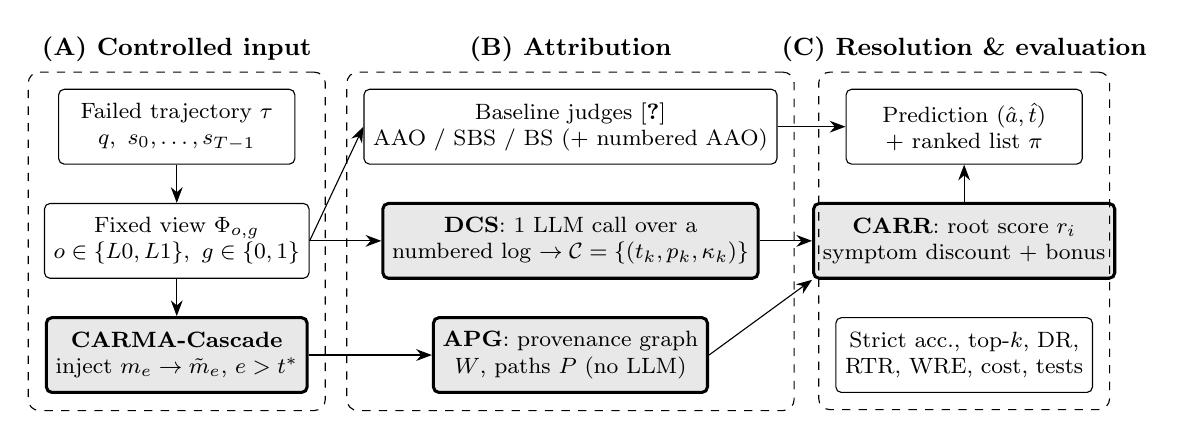
\begin{tikzpicture}[
  box/.style={draw, rounded corners=2pt, align=center, minimum width=3.0cm, minimum height=0.95cm, font=\footnotesize},
  new/.style={box, fill=gray!18, line width=1.1pt},
  grp/.style={draw, dashed, rounded corners=4pt, inner sep=6pt},
  >={Stealth[length=2mm]}]
\node[box] (traj) at (0,0) {Failed trajectory $\tau$\\ $q,\ s_0,\dots,s_{T-1}$};
\node[box] (view) at (0,-1.45) {Fixed view $\Phi_{o,g}$\\ $o\in\{L0,L1\},\ g\in\{0,1\}$};
\node[new] (cas)  at (0,-2.9) {\textbf{CARMA-Cascade}\\ inject $m_e\to\tilde m_e$, $e>t^*$};
\node[box] (base) at (5.0,0) {Baseline judges~\cite{zhang2025whowhen}\\ AAO / SBS / BS (+ numbered AAO)};
\node[new] (dcs)  at (5.0,-1.45) {\textbf{DCS}: 1 LLM call over a\\ numbered log $\to \mathcal{C}=\{(t_k,p_k,\kappa_k)\}$};
\node[new] (apg)  at (5.0,-2.9) {\textbf{APG}: provenance graph\\ $W$, paths $P$ (no LLM)};
\node[box] (pred) at (10.0,0) {Prediction $(\hat a,\hat t)$\\ + ranked list $\pi$};
\node[new] (carr) at (10.0,-1.45) {\textbf{CARR}: root score $r_i$\\ symptom discount + bonus};
\node[box] (eval) at (10.0,-2.9) {Strict acc., top-$k$, DR,\\ RTR, WRE, cost, tests};
\node[grp, fit=(traj)(cas), label={[font=\small\bfseries]above:(A) Controlled input}] {};
\node[grp, fit=(base)(apg), label={[font=\small\bfseries]above:(B) Attribution}] {};
\node[grp, fit=(pred)(eval), label={[font=\small\bfseries]above:(C) Resolution \& evaluation}] {};
\draw[->] (traj) -- (view); \draw[->] (view) -- (cas);
\draw[->] (view.east) -- (base.west); \draw[->] (view.east) -- (dcs.west); \draw[->] (cas.east) -- (apg.west);
\draw[->] (base.east) -- (pred.west); \draw[->] (dcs.east) -- (carr.west); \draw[->] (apg.east) -- (carr.south west);
\draw[->] (carr) -- (pred);
\end{tikzpicture}
\caption{CARMA workflow. (A) A failed trajectory is rendered under a fixed observability level and ground-truth setting, optionally after cascade injection. (B) Baseline judges produce a single prediction; DCS produces a scored candidate list with one LLM call; the Artifact Provenance Graph is built deterministically from the trace. (C) CARR combines both into a root score, and all predictions are scored with the same strict metrics, distraction rate, rollback-trigger metrics and cost. Shaded, thick-bordered boxes are new components.}
\label{fig:workflow}
\end{figure*}


\begin{table}[t]
\centering
\caption{Notation.}
\label{tab:notation}
\footnotesize
\begin{tabular}{@{}l@{\hspace{4pt}}p{0.62\columnwidth}@{}}
\toprule
Symbol & Meaning \\
\midrule
$q, y^*$ & task query and correct final answer \\
$s_t=(a_t,m_t)$ & step $t$: agent and message, $t=0..T{-}1$ \\
$t^*, a^*$ & annotated decisive step and agent \\
$o, g$ & observability level; ground-truth flag \\
$\mathcal{C}=\{(t_k,p_k,\kappa_k)\}$ & DCS candidates: step, probability, tag \\
$\alpha(m)$ & set of concrete artifacts extracted from text $m$ \\
$\mathrm{org}(x)$ & first step at which artifact $x$ appears \\
$W\in[0,1]^{T\times T}$ & provenance edge weights, $W_{ji}>0\Rightarrow j<i$ \\
$P_{ji}$ & strongest dependency path strength $j\rightsquigarrow i$ \\
$\gamma,\beta$ & CARR symptom-discount and explanation-bonus weights \\
$r_i$ & CARR root score of candidate step $i$ \\
$E, e$ & error set and injected step in CARMA-Cascade \\
\bottomrule
\end{tabular}
\end{table}

\textbf{Dense Candidate Scoring (DCS).} Given $x$, one LLM call with the numbered log returns up to $K=5$ candidates in JSON,
\begin{equation}
\mathrm{DCS}(x)=\mathcal{C}=\{(t_k,p_k,\kappa_k)\}_{k=1}^{K'},\quad K'\le K,\quad \textstyle\sum_k p_k\le 1,
\end{equation}
where $p_k$ is the judge's probability that $t_k$ is the decisive error and $\kappa_k\in\{\text{origin},\text{propagated}\}$. The prompt defines the decisive error as the earliest error whose correction would most likely have produced success and warns that later steps may look wrong only because they reused an earlier wrong result. Out-of-range steps are dropped, duplicates are merged by summing $p$, and $p$ is renormalised if $\sum_k p_k>1$. The agent of each candidate is read from the log ($a_{t_k}$), not from the judge, which removes agent-name hallucination. So DCS differs from All-at-Once in three ways at once: the log is numbered, the prompt is different, and the output is a list. Table~\ref{tab:decomp} separates the three.

\textbf{Artifact Provenance Graph (APG).} Let $\alpha(m)$ extract concrete artifacts from a message: numbers of at least two characters (excluding 0--12 and common years), URLs, file names, identifiers containing an underscore or camel case (at least six characters), and quoted strings of 4--60 characters. Artifacts appearing in $q$ or $y^*$ are marked as \emph{given} and never attributed to an agent. Each remaining artifact has an origin $\mathrm{org}(x)=\min\{t: x\in\alpha(m_t)\}$. The edge weight from $j$ to $i>j$ is the share of step $i$'s reused artifacts that originate at $j$:
\begin{equation}
W_{ji}=\frac{|\{x\in\alpha(m_i):\mathrm{org}(x)=j\}|}{|\{x\in\alpha(m_i):\mathrm{org}(x)<i,\ x \text{ not given}\}|}.
\end{equation}
Because edges only point forward in time, $W$ is a DAG. The strength of the strongest dependency path is computed by dynamic programming over increasing $i$,
\begin{equation}
P_{ji}=\min\Big(1,\ \max\big(W_{ji},\ \max_{j<m<i} P_{jm}W_{mi}\big)\Big),\label{eq:path}
\end{equation}
which costs $O(T^3)$ in the worst case (below 3\,ms for $T=130$).

\textbf{Cascade-Aware Root Resolution (CARR).} CARR treats each candidate as a possible root and scores it by how likely it is to be erroneous, how unlikely it is to be merely inherited from an erroneous ancestor, and how much downstream erroneous behaviour it explains:
\begin{equation}
r_i=p_i\prod_{\substack{(j,p_j)\in\mathcal{C}\\ j<i}}\big(1-\gamma\,p_jP_{ji}\big)\Big(1+\beta\!\!\sum_{\substack{(k,p_k)\in\mathcal{C}\\ k>i}}\!\! p_kP_{ik}\Big).\label{eq:carr}
\end{equation}
The product is a noisy-OR style \emph{symptom discount}: if an earlier candidate $j$ is likely wrong ($p_j$ high) and $i$ demonstrably reuses $j$'s artifacts ($P_{ji}$ high), then $i$'s apparent error is better explained by $j$. The sum is an \emph{explanation bonus} for candidates whose artifacts flow into other likely-erroneous steps. The prediction is $\hat t=\arg\max_i r_i$ (ties to the earlier step), $\hat a=a_{\hat t}$, and the full CARR order gives the ranked list $\pi$. With $\gamma=\beta=0$ CARR reduces to DCS top-1, and replacing $P$ with the complete temporal graph ($P_{ji}=1$ for all $j<i$) gives a positional ``prefer earlier'' heuristic; both are ablations. Algorithm~\ref{alg:carma} summarises inference.

\begin{algorithm}[t]
\caption{CARMA inference (DCS + APG + CARR)}\label{alg:carma}
\footnotesize
\begin{algorithmic}[1]
\Require trajectory $\tau$, view $(o,g)$, judge LLM, $K,\gamma,\beta$
\State $\mathcal{C}\gets$ \textsc{ParseJSON}(LLM(\textsc{DCSPrompt}($\Phi_{o,g}(\tau),K$))) \Comment{1 call}
\State drop out-of-range steps; merge duplicates; renormalise $p$ if $\sum p>1$
\If{$\mathcal{C}=\emptyset$} \Return (None, None, [ ]) \EndIf
\State $\mathrm{org}\gets\{x\mapsto -1: x\in\alpha(q)\cup\alpha(y^*)\}$; $W\gets 0^{T\times T}$
\For{$i=0$ \textbf{to} $T-1$}
  \State $R\gets\{x\in\alpha(m_i):\mathrm{org}(x)\ge 0\}$
  \For{$x\in R$} $W_{\mathrm{org}(x),i}\mathrel{+}=1/|R|$ \EndFor
  \For{$x\in\alpha(m_i)$ with $x\notin\mathrm{org}$} $\mathrm{org}(x)\gets i$ \EndFor
\EndFor
\State compute $P$ by Eq.~(\ref{eq:path})
\For{$(i,p_i)\in\mathcal{C}$} compute $r_i$ by Eq.~(\ref{eq:carr}) \EndFor
\State $\pi\gets$ candidates sorted by $(-r_i, i)$; $\hat t\gets\pi_1$; $\hat a\gets a_{\hat t}$
\State \Return $(\hat a,\hat t,\pi)$
\end{algorithmic}
\end{algorithm}

\textbf{Training and optimisation.} CARMA has no trainable parameters. The judge is used zero-shot at temperature 0. The two scalars $\gamma=1$ and $\beta=0.5$ were fixed a priori from the semantics of Eq.~(\ref{eq:carr}) ($\gamma=1$ makes the discount a proper noisy-OR; $\beta=0.5$ lets explanation at most modestly reorder candidates) and recorded before any DCS or CARR result was inspected. Their sensitivity is reported in Section~\ref{sec:ablation} but is not used to select the headline configuration.

\textbf{Inference and execution.} At run time a failed trajectory triggers one DCS call; the APG and CARR run in milliseconds on the CPU. The output is a responsible agent, a decisive step, and a ranked list usable as a rollback schedule: a controller would first roll back to $\pi_1$, and if the re-run still fails, to the next candidate. Because DCS is a single call, latency equals one judge call, compared with up to $T$ sequential calls for SBS and about $\log_2 T$ for BS.

\textbf{Technical novelty and justification.} DCS shares the numbered log with A2P~\cite{west2025a2p} and the observation that judges miscount unnumbered logs with DoVer~\cite{ma2025dover}; we do not claim numbering as a contribution and measure its share of the gain explicitly. What DCS adds is a scored list with origin/propagated tags obtained in one call, which can be evaluated as a ranking and used as a rollback schedule. Compared with GraphTracer, CHIEF and FALAT~\cite{zhang2025graphtracer,wang2026chief,rafi2026falat}, the APG is read deterministically from artifacts in the trace, costs no LLM calls or training, and works as a plug-in over any method that emits candidate probabilities; root/symptom separation is computed outside the LLM, so it cannot be hallucinated and can be audited edge by edge. Compared with conformal sets~\cite{feng2026conformal}, CARR orders candidates by causal role rather than calibrating set size, and the two are complementary. The fixed protocol and controls target G1; CARMA-Cascade, the distraction rate and CARR's symptom discount target G2; the rollback-trigger metrics, the rollback schedule and cost accounting target G3.

\section{Experimental Results and Discussion}\label{sec:exp}
\subsection{Experimental Setup and Implementation}\label{sec:setup}
\textbf{Environment.} All components are implemented in Python~3.12 with the standard library only (plus \texttt{matplotlib} for figures), in a single code base shared by the baselines and the proposed method, so that runs differ only in the attribution procedure. No GPU is required because all LLM inference is served by an API. The judge is \texttt{ministral-14b-latest} (Mistral AI, 262k-token context) at temperature 0, with a maximum of 1024 output tokens for the baselines (the official default) and 2048 for DCS's JSON. A second, smaller backbone, \texttt{open-mistral-nemo}, tests whether conclusions transfer across models, and \texttt{ministral-8b-latest} (temperature 0.7) is used only to inject cascade errors so that neither judge evaluates its own rewrites. The free API tier limits each model to two requests and 40k tokens per minute, which determined the scope described below.

\textbf{Protocol and reproducibility.} Every LLM response is cached on disk under a SHA-256 key of the model, prompts and generation configuration. Each run writes one JSON line per trajectory (prediction, raw response, calls, input and output tokens, latency), and all tables and figures in this section are generated from these files by \texttt{scripts/make\_tables.py}, \texttt{scripts/extra\_analysis.py} and \texttt{scripts/make\_figures.py}. All settings, including the backbone, $K=5$, $\gamma=1$, $\beta=0.5$, the artifact types and the cascade seed, were fixed in a pre-registration file (\texttt{research/preregistration.md}) before any DCS or CARR result was inspected; the file was first committed together with the first results, so the repository history alone cannot prove this order; the numbered All-at-Once and $K{=}1$ controls and the flattening check were added afterwards and are post-hoc. The main condition is observability L0 with ground truth ($g=1$), the default setting of~\cite{zhang2025whowhen}. Every comparison is paired on the trajectories that all compared methods completed. We report unadjusted $p$-values; for the decomposition (three tests per judge), the Holm-adjusted values of the significant steps stay below 0.05 (largest: $0.016$ for the 14B DCS prompt), while the cascade tests, the sensitivity sweep and the flattening check are exploratory.

\textbf{Run-to-run variability.} API inference at temperature 0 is not bit-reproducible, and the control runs (numbered All-at-Once, DCS with $K{=}1$, hand-crafted and cascade completions) were made about a week after the main runs. We therefore re-ran All-at-Once on a fixed random sample of 20 algorithm-generated logs: the re-run agrees with the logged prediction on the step in 15 of 20 logs and on the agent in 19 of 20, and is correct on 4 versus 3 logs. A quarter of step predictions can thus change between two calls on identical input; we did not repeat this check for DCS. Differences of a few points between single runs can be run-to-run noise, so we rely on paired tests rather than on point differences.

\textbf{Completed runs.} With \texttt{ministral-14b}: All-at-Once, numbered All-at-Once, DCS with $K{=}1$ and DCS with $K{=}5$ on all 126 algorithm-generated logs; All-at-Once, numbered All-at-Once and DCS on all 111 CARMA-Cascade logs; All-at-Once and DCS on 57 of the 58 hand-crafted logs; Binary Search on a fixed random sample of 60 algorithm-generated logs. With \texttt{open-mistral-nemo}: the same algorithm-generated, cascade and hand-crafted runs, without Binary Search. Step-by-Step (up to $T$ calls per log), the setting without ground truth ($g=0$) and observability L1 are implemented but were not run within the API budget.

\textbf{Implemented components.} We implemented (i) the three baselines of~\cite{zhang2025whowhen} with their official prompts, plus All-at-Once on the numbered log, (ii) DCS (with $K=5$ and $K=1$), the APG and CARR (Algorithm~\ref{alg:carma}), (iii) the CARMA-Cascade construction, and (iv) the evaluation protocol. From one DCS run we derive, without further calls, DCS top-1, two ablations (earliest candidate; earliest candidate the judge itself tagged as ``origin''), CARR with a temporal graph, and full CARR.

\subsection{Evaluation Metrics}
We adopt the agent-level and step-level accuracy of~\cite{zhang2025whowhen}, the tolerance accuracy used in its Table~2, top-$k$ accuracy as used for candidate ranking in later work~\cite{feng2026conformal}, and add metrics for G2 and G3 (Table~\ref{tab:metrics}).

\begin{table}[t]
\centering
\caption{Evaluation metrics. $\mathbf{1}[\cdot]$ is the indicator; averages are over trajectories.}
\label{tab:metrics}
\footnotesize
\setlength{\tabcolsep}{2.5pt}
\begin{tabular}{@{}p{1.35cm}p{3.6cm}p{2.9cm}@{}}
\toprule
Metric & Definition & Purpose (objective) \\
\midrule
Agent acc. & $\mathbf{1}[\hat a=a^*]$ (exact, case- and suffix-normalised) & who failed~\cite{zhang2025whowhen} (O1) \\
Step acc. & $\mathbf{1}[\hat t=t^*]$ (exact integer match) & when it failed~\cite{zhang2025whowhen} (O1, O2) \\
Lenient acc. & $\mathbf{1}[\mathrm{str}(t^*)\sqsubseteq\mathrm{str}(\hat t)]$ (substring, official script) & reproduction only (O1) \\
Acc@$\pm k$ & $\mathbf{1}[|\hat t-t^*|\le k]$ & near misses~\cite{zhang2025whowhen} \\
Top-$k$ & $\mathbf{1}[t^*\in\{\pi_1..\pi_k\}]$ & candidate quality~\cite{feng2026conformal} \\
DR & $\mathbf{1}[\hat t\in E_{\text{inj}}]$ on CARMA-Cascade & distraction (O2) \\
ECE & $\sum_b \frac{n_b}{n}|\bar p_b-\mathrm{acc}_b|$ over confidence bins & calibration of DCS (O2) \\
RTR & $\mathbf{1}[\hat t\le t^*]$ & rollback re-generates $t^*$ (O3) \\
WRE & $\mathbb{E}[(t^*-\hat t)/T\mid\hat t\le t^*]$ & correct work discarded (O3) \\
Schedule & attempts and re-executed steps until some $\pi_k\le t^*$ & ranked list as rollback plan (O3) \\
Cost & calls, input/output tokens, latency per trajectory & efficiency (O3) \\
\bottomrule
\end{tabular}
\end{table}

Step accuracy is the primary metric because it is what both the base paper and later work report and what the proposed method claims to improve; agent accuracy is secondary because the agent is determined by the step in our method. The lenient metric reproduces the official \texttt{evaluate.py}, which tests \texttt{actual\_step in predicted\_step} on strings; we report it only to explain differences from published numbers. DR directly measures G2; we report it together with its \emph{pre-injection} level (how often the method already predicted the same step $e$ on the original log) and the chance level $\mathbb{E}[1/T]$. RTR and WRE score a prediction as a rollback trigger~\cite{ma2025dover,feng2026conformal}. The schedule metric tries $\pi_1,\pi_2,\dots$ (then step~0) and counts attempts and re-executed steps (as a multiple of $T$) until a rollback point at or before $t^*$ is reached. These are offline proxies because Who\&When logs cannot be re-executed. Statistical uncertainty is reported as 95\% bootstrap confidence intervals over trajectories (2,000 resamples) and, for paired differences, as paired-bootstrap intervals (5,000 resamples); paired method comparisons use the exact two-sided McNemar test on per-trajectory correctness.

\subsection{Reproducibility of the Base Paper}
We re-implemented the attribution pipeline of~\cite{zhang2025whowhen} from its public code and prompts: the same trajectory rendering, the same All-at-Once, Step-by-Step and Binary Search prompts, the same parsing of the ``Agent Name / Step Number'' answer, and the same ground-truth line in the prompt. Table~\ref{tab:repro} compares the published GPT-4o results with our runs.

\begin{table}[t]
\centering
\caption{Reproduction of the Who\&When baselines (with ground truth). Reported: GPT-4o, Table~1 of~\cite{zhang2025whowhen}. Reproduced: \texttt{ministral-14b}; strict / lenient (official substring) scoring.}
\label{tab:repro}
\footnotesize
\setlength{\tabcolsep}{3pt}
\begin{tabular}{@{}llccccc@{}}
\toprule
 & & \multicolumn{2}{c}{Reported} & \multicolumn{3}{c}{Reproduced} \\
\cmidrule(lr){3-4}\cmidrule(lr){5-7}
Subset & Method & Agent & Step & $n$ & Agent & Step (strict / len.) \\
\midrule
Alg. & AAO & 54.3 & 12.5 & 126 & 52.4 & 14.3 / 15.9 \\
Alg. & SBS & 35.2 & 25.5 & -- & \multicolumn{2}{c}{not run} \\
Alg. & BS & 44.1 & 24.0 & -- & \multicolumn{2}{c}{not run} \\
Hand & AAO & 55.2 & 5.3 & 6 & 83.3 & 0.0 / 0.0 \\
Hand & SBS & 34.5 & 7.0 & -- & \multicolumn{2}{c}{not run} \\
Hand & BS & 51.7 & 6.9 & -- & \multicolumn{2}{c}{not run} \\
\bottomrule
\end{tabular}
\end{table}

The reproduced All-at-Once judge reaches 52.4\% agent accuracy (reported 54.3\%) and 14.3\% strict step accuracy (reported 12.5\%); under the official substring scoring the step accuracy is 15.9\%. The reported step value lies inside our 95\% bootstrap interval [7.9, 20.6]. The second backbone gives 49.2\% and 13.5\% (Table~\ref{tab:backbone}). We consider the All-at-Once baseline reproduced. Binary Search, run on a fixed random sample of 60 algorithm-generated logs, reaches 20.0\% strict step accuracy (reported 24.0\%, inside our interval [10.0, 30.0]) but only 35.0\% agent accuracy (reported 44.1\%). On the hand-crafted logs, All-at-Once reaches 3.5\% step and 59.6\% agent accuracy (reported 5.3\% and 55.2\%). Step-by-Step, which needs up to $T$ calls per log, was not run within the API budget; we report its published values only.

\textbf{An indexing artefact in the baseline protocol.} The official All-at-Once prompt asks for a 0-based step index over an unnumbered log. Neither judge ever predicts step~0 (0 of 126 logs for both), although $t^*=0$ in 20 logs, so All-at-Once is 0\% accurate on those logs; the 14B judge answers ``step 1'' in 43 of 126 logs. In only 26.2\% (14B) and 23.8\% (Nemo) of logs is the agent it names the agent who actually speaks at the step it predicts. Its step errors are skewed late ($+1$: 17.5\% vs.\ $-1$: 7.1\%; Fig.~\ref{fig:offsets}), consistent with counting from one, but shifting every prediction by $-1$ only raises its accuracy to 17.5\%, so miscounting is part of the explanation, not all of it. Agent accuracy (about 50\%) is a more faithful summary of the unnumbered judge than step accuracy, and step-level comparisons with this baseline mostly measure whether the judge can locate positions at all. In other words, the published baseline's step accuracy depends on log formatting as much as on reasoning (G1).

\textbf{Deviation log.} (i) \emph{Backbone.} The published runs used GPT-4o; we used open-weight Mistral models (Section~\ref{sec:setup}). (ii) \emph{Scoring.} Strict integer matching is primary; the substring score is reported only for comparison. The 1.6-point gap on this subset is small because most algorithm-generated logs have fewer than ten steps; it grows with log length. (iii) \emph{Scope.} Binary Search is evaluated on a fixed random sample of 60 algorithm-generated logs because it needs about $\log_2 T$ calls per log at two requests per minute; Step-by-Step (up to $T$ calls per log) was not run. (iv) \emph{Long logs.} One hand-crafted log failed after API retries and is excluded from the paired hand-crafted comparison. (v) \emph{Answer parsing.} The official script falls back to a random choice when no step can be parsed; we record the prediction as missing and score it as wrong, which can only lower our numbers. (vi) \emph{Random reference.} The base paper reports 19.06\% random step accuracy on this subset; we report the analytic $\mathbb{E}[1/T]=12.0\%$ of a uniform guess; the definitions differ.

\subsection{Results and Comparative Analysis}
\textbf{Main result.} Table~\ref{tab:main_full} compares the reproduced baseline with the proposed method under the main condition (L0, $g=1$) on all 126 algorithm-generated trajectories. DCS raises strict step accuracy from 14.3\% to 40.5\%, a paired difference of $+26.2$ points (95\% paired-bootstrap CI [16.7, 35.7]); of the 45 trajectories on which exactly one method is correct, DCS wins 39 and All-at-Once 6 (exact McNemar $p<0.001$). Agent accuracy rises less, from 52.4\% to 57.1\%; because DCS reads the agent off its predicted step, this is not independent evidence.

\begin{table*}[t]
\centering
\caption{Algorithm-generated subset, all trajectories: baseline vs. proposed (L0, with ground truth) ($n=126$).}
\label{tab:main_full}
\footnotesize
\setlength{\tabcolsep}{4pt}
\begin{tabular}{@{}lcccccccccc@{}}
\toprule
Method & Agent & Step & 95\% CI & Acc@$\pm$1 & Top-3 & RTR & WRE$\downarrow$ & Calls & Tokens & $p$ vs AAO \\
\midrule
All-at-Once~\cite{zhang2025whowhen} & 52.4 & 14.3 & [7.9, 20.6] & 38.9 & 14.3 & 48.4 & 25.7 & 1.0 & 4.1k & -- \\
DCS top-1 (ours) & 57.1 & 40.5 & [31.7, 49.2] & 56.3 & 71.4 & 90.5 & 21.7 & 1.0 & 4.0k & $<$0.001 \\
\textbf{DCS + CARR (ours)} & 57.1 & 40.5 & [31.7, 49.2] & 56.3 & 70.6 & 90.5 & 21.7 & 1.0 & 4.0k & $<$0.001 \\
\bottomrule
\end{tabular}
\end{table*}

\textbf{Trivial baselines.} Always predicting step~0 is correct in 15.9\% of trajectories, slightly above the reproduced All-at-Once, and it has RTR = 100\% by construction while discarding 37\% of the trajectory on average. A uniformly random step gives 12.0\% and RTR 44.7\%. DCS is 24.6 points above the step-0 rule in step accuracy and discards less work (WRE 21.7\%); 15 of its 51 correct predictions are on the 20 logs with $t^*=0$.

\textbf{Where the gain comes from.} DCS changes three things relative to All-at-Once: the log is numbered, the prompt defines the decisive error and warns about propagation, and the output is a scored list. Table~\ref{tab:decomp} adds one change per row on the same trajectories. First, numbering the log is the largest single change for the main judge: it raises All-at-Once from 14.3\% to 31.0\% ($+16.7$ points, $p<0.001$), the gain holds on the 106 logs whose decisive step is not step~0, and it removes the inability to name step~0 (12 such predictions instead of none). With the second judge the same change gives $+8.7$ points with $p=0.061$. This agrees in direction with the numbering ablation of A2P~\cite{west2025a2p}, which reports $+29.7$ points, and we do not claim it as a contribution. Second, the DCS prompt adds a further $+13.5$ points with the main judge ($p=0.008$) and $+22.2$ points with the second ($p<0.001$), but part of this comes from a shift towards early steps: with $K{=}1$ the judges predict step~0 in 31 (14B) and 38 (Nemo) of 126 logs, while step~0 is decisive in 20. On the logs with $t^*>0$ the prompt's gain over numbered All-at-Once is not significant for the main judge (37.7\% vs.\ 32.1\%, $p=0.33$) but is for the second (37.7\% vs.\ 23.6\%, $p=0.01$). The part of the DCS gain that goes beyond numbering is judge-dependent and partly an earliness bias, which matters for the cascade results below, since a judge that prefers early steps is less exposed to errors injected late. Third, asking for a scored list of five candidates instead of one step does not change top-1 accuracy for either judge ($-4.0$ and $-3.2$ points, $p\ge0.35$). The list is useful as a ranking and as a rollback schedule, not as a way to improve the first answer.

\begin{table*}[t]
\centering
\caption{Where does the gain come from? One factor added per row on the same trajectories (algorithm-generated, L0, $g{=}1$). $\Delta$: paired difference to the row above with 95\% paired-bootstrap CI; $p$: exact McNemar against the row above. $t^*{>}0$: step accuracy on the logs whose decisive step is not step~0 (McNemar against the row above). $\hat t{=}0$: number of logs on which the method predicts step~0 (gold: 20 of 126).}
\label{tab:decomp}
\footnotesize
\setlength{\tabcolsep}{2.5pt}
\begin{tabular}{@{}llcccccc@{}}
\toprule
Judge & Prompt / format & $n$ & Step & $\Delta$ [95\% CI] & $p$ & $t^*{>}0$ ($p$) & $\hat t{=}0$ \\
\midrule
14B & AAO, unnumbered (official) & 126 & 14.3 & -- & -- & 17.0 (--) & 0 \\
14B & AAO + step numbers & 126 & 31.0 & +16.7 [+9.5, +23.8] & $<$0.001 & 32.1 ($<$0.001) & 12 \\
14B & DCS prompt, single step ($K{=}1$) & 126 & 44.4 & +13.5 [+4.8, +23.0] & 0.008 & 37.7 (0.33) & 31 \\
14B & DCS, scored list ($K{=}5$), top-1 & 126 & 40.5 & -4.0 [-11.1, +2.4] & 0.359 & 34.0 (0.42) & 38 \\
\midrule
Nemo & AAO, unnumbered (official) & 126 & 13.5 & -- & -- & 16.0 (--) & 0 \\
Nemo & AAO + step numbers & 126 & 22.2 & +8.7 [+0.8, +17.5] & 0.061 & 23.6 (0.17) & 5 \\
Nemo & DCS prompt, single step ($K{=}1$) & 126 & 44.4 & +22.2 [+12.7, +31.7] & $<$0.001 & 37.7 (0.01) & 38 \\
Nemo & DCS, scored list ($K{=}5$), top-1 & 126 & 41.3 & -3.2 [-11.9, +5.6] & 0.585 & 40.6 (0.65) & 18 \\
\bottomrule
\end{tabular}
\end{table*}

\begin{figure}[t]
\centering
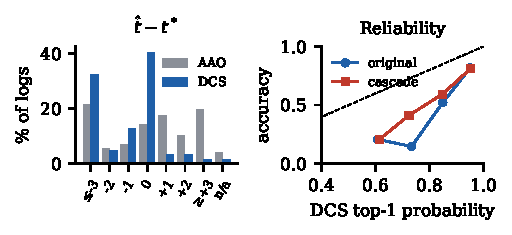
\includegraphics[width=\columnwidth]{figures/offsets_calibration.pdf}
\caption{Left: signed step error $\hat t-t^*$ of All-at-Once and DCS (\texttt{ministral-14b}, 126 logs). Right: reliability of the DCS top-1 probability on original and cascaded logs (bins with $\ge5$ logs); the dashed line is perfect calibration.}
\label{fig:offsets}
\end{figure}

\textbf{Comparison with Binary Search.} Table~\ref{tab:main_sub} compares all methods run with the main judge on the same 60 logs. Binary Search (20.0\%) is above All-at-Once (11.7\%), as in the base paper, but its advantage is not significant ($p=0.23$). DCS reaches 33.3\%, 13.3 points above Binary Search with a third of the calls, but on 60 logs this difference is not significant either (14 to 6 discordant logs, $p=0.12$); numbered All-at-Once reaches 26.7\% on the same sample ($p=0.45$ against Binary Search). The sample is too small to rank these three methods, and we do not claim that DCS beats Binary Search.

\begin{table*}[t]
\centering
\caption{Paired comparison of all methods on the fixed 60-trajectory algorithm-generated subset ($n=4$).}
\label{tab:main_sub}
\footnotesize
\setlength{\tabcolsep}{4pt}
\begin{tabular}{@{}lcccccccccc@{}}
\toprule
Method & Agent & Step & 95\% CI & Acc@$\pm$1 & Top-3 & RTR & WRE$\downarrow$ & Calls & Tokens & $p$ vs AAO \\
\midrule
All-at-Once~\cite{zhang2025whowhen} & 75.0 & 0.0 & [0.0, 0.0] & 50.0 & 0.0 & 0.0 & -- & 1.0 & 2.5k & -- \\
Binary Search~\cite{zhang2025whowhen} & 0.0 & 0.0 & [0.0, 0.0] & 75.0 & 0.0 & 25.0 & 12.5 & 3.0 & 4.1k & 1.000 \\
DCS top-1 (ours) & 75.0 & 75.0 & [25.0, 100.0] & 75.0 & 100.0 & 100.0 & 6.2 & 1.0 & 2.5k & 0.250 \\
\textbf{DCS + CARR (ours)} & 75.0 & 75.0 & [25.0, 100.0] & 75.0 & 100.0 & 100.0 & 6.2 & 1.0 & 2.5k & 0.250 \\
\bottomrule
\end{tabular}
\end{table*}

\textbf{Relation to the state of the art.} A2P~\cite{west2025a2p} reports 47.46\% step accuracy on this subset, above our 40.5\%, and the base paper reports 25.5\% for Step-by-Step with GPT-4o. The numbers are not directly comparable: both use larger proprietary backbones, A2P uses multi-stage causal prompting, and Step-by-Step needs up to $T$ calls, while DCS uses a 14B open-weight judge and a single call. We do not claim state-of-the-art accuracy.

\textbf{The candidate list as a ranking and a rollback schedule (O3).} The gold step is among the top three DCS candidates in 71.4\% of trajectories and among all candidates (on average 4.4) in 84.9\%; the corresponding numbers for the second judge are 68.3\% and 82.5\%. Rolling back to the step predicted by DCS would re-generate the decisive error in 90.5\% of trajectories, against 48.4\% for All-at-Once, while discarding slightly less correct work (WRE 21.7\% vs.\ 25.7\%). Part of this RTR comes from early predictions: DCS predicts three or more steps before $t^*$ in 32.5\% of logs (Fig.~\ref{fig:offsets}), which is why RTR is reported only with WRE. Used as a schedule, the DCS list reaches a rollback point at or before $t^*$ on the first attempt in 92.1\% of logs and after 1.25 attempts on average, against 52.4\% and 1.48 for All-at-Once followed by step~0.

\textbf{Second backbone.} The same ordering holds with \texttt{open-mistral-nemo} (Table~\ref{tab:backbone}): All-at-Once 13.5\%, DCS 41.3\%, a paired gain of $+27.8$ points [17.5, 38.1] (43 to 8 discordant trajectories, $p<0.001$). The two judges agree on the DCS top-1 step in 61.9\% of logs; at least one is correct in 51.6\% and both in 30.2\%.

\begin{table*}[t]
\centering
\caption{Second backbone (\texttt{open-mistral-nemo}), algorithm-generated subset ($n=126$).}
\label{tab:backbone}
\footnotesize
\setlength{\tabcolsep}{4pt}
\begin{tabular}{@{}lcccccccccc@{}}
\toprule
Method & Agent & Step & 95\% CI & Acc@$\pm$1 & Top-3 & RTR & WRE$\downarrow$ & Calls & Tokens & $p$ vs AAO \\
\midrule
All-at-Once~\cite{zhang2025whowhen} & 49.2 & 13.5 & [7.9, 19.0] & 33.3 & 13.5 & 50.8 & 23.3 & 1.0 & 4.3k & -- \\
DCS top-1 (ours) & 62.7 & 41.3 & [32.5, 50.0] & 53.2 & 68.3 & 84.1 & 17.7 & 1.0 & 4.1k & $<$0.001 \\
\textbf{DCS + CARR (ours)} & 62.7 & 39.7 & [31.0, 48.4] & 51.6 & 67.5 & 84.1 & 18.7 & 1.0 & 4.1k & $<$0.001 \\
\bottomrule
\end{tabular}
\end{table*}

\textbf{Robustness to cascading errors (G2).} Table~\ref{tab:cascade} and Fig.~\ref{fig:cascade} report CARMA-Cascade, where each trajectory carries one additional, independently injected error after the annotated decisive step. A manipulation check first confirms that the judge notices the injected errors. With the 14B judge, the injected step appears in the DCS list in 85.6\% of cascaded logs against 64.0\% of the same logs before injection, and its mean probability rises from 0.045 to 0.104. The judge rarely promotes it to first place, though. DCS accuracy is unchanged by the injection (45.0\% to 45.9\%, McNemar $p=1.0$), and its distraction rate rises from 1.8\% before injection to 5.4\%, well below the chance level of 12.1\%. All-at-Once loses more: its accuracy falls from 16.2\% to 9.9\% (4 to 11 discordant logs, $p=0.12$) and its distraction rate rises from 6.3\% to 11.7\%. The smaller judge is less robust with DCS. Its accuracy falls from 45.9\% to 37.8\% (5 to 14, $p=0.064$), its distraction rate rises from 3.6\% to 14.4\%, above chance, and the injected step receives a mean probability of 0.163 (0.071 before injection). Neither drop is significant at the 5\% level on 111 logs, and given the run-to-run variability reported in Section~\ref{sec:setup}, changes of this size may partly be noise.

\textbf{Is the robustness just earliness?} Table~\ref{tab:decomp} showed that the 14B DCS judge prefers early steps, and a judge that prefers early steps is naturally less exposed to an error injected late. To test this we ran numbered All-at-Once on the same cascaded logs. It does not hold up. With the main judge, numbered All-at-Once falls from 31.5\% to 21.6\% (5 to 16 discordant logs, $p=0.027$) and picks the injected step in 45.9\% of cascaded logs, up from 9.0\% of the original logs. DCS picks it in 5.4\% of the same logs (46 to 1 discordant logs, $p<0.001$). With the second judge, numbered All-at-Once keeps its accuracy (23.4\% to 22.5\%, $p=1.0$) but picks the injected step in 33.3\% of cascaded logs, up from 11.7\%, against 14.4\% for DCS (27 to 6 discordant logs, $p<0.001$). Numbering does not protect a judge from a later error. The DCS prompt, which defines the decisive error and warns that later steps may only expose it, cuts the distraction rate by a factor of 2.3 (weaker judge) to 8.5 (stronger judge). The control also shows that accuracy alone can hide distraction, because the injected step mostly attracts predictions that were already wrong.

\textbf{Limits of the cascade design.} The injected error is independent of $t^*$, so CARMA-Cascade tests distraction by a later error. It does not test whether a method can separate a root from symptoms the root caused, which is what CARR's discount targets. And once a second error is present, correcting $t^*$ alone may no longer turn the run into a success, so $t^*$ is the decisive step of the original failure rather than a re-annotated label.

\begin{table}[t]
\centering
\caption{CARMA-Cascade: step accuracy on the original logs vs.\ the same logs with one injected downstream error, and distraction rate (DR, share of predictions blaming the injected step).}
\label{tab:cascade}
\footnotesize
\setlength{\tabcolsep}{3pt}
\begin{tabular}{@{}llcccccc@{}}
\toprule
Judge & Method & $n$ & Orig. & Cascade & $\Delta$ ($p$) & DR pre & DR$\downarrow$ \\
\midrule
14B & All-at-Once & 58 & 12.1 & 6.9 & -5.2 (0.45) & 8.6 & 13.8 \\
14B & DCS top-1 (ours) & 111 & 45.0 & 45.9 & +0.9 (1.00) & 1.8 & 5.4 \\
14B & DCS + CARR, temporal graph & 111 & 45.0 & 45.9 & +0.9 (1.00) & 1.8 & 5.4 \\
14B & \textbf{DCS + CARR (ours)} & 111 & 45.0 & 45.9 & +0.9 (1.00) & 1.8 & 5.4 \\
Nemo & DCS top-1 (ours) & 85 & 48.2 & 37.6 & -10.6 (0.04) & 2.4 & 15.3 \\
Nemo & DCS + CARR, temporal graph & 85 & 47.1 & 36.5 & -10.6 (0.04) & 2.4 & 15.3 \\
Nemo & \textbf{DCS + CARR (ours)} & 85 & 47.1 & 37.6 & -9.4 (0.06) & 2.4 & 15.3 \\
\bottomrule
\end{tabular}
\end{table}

\begin{figure}[t]
\centering
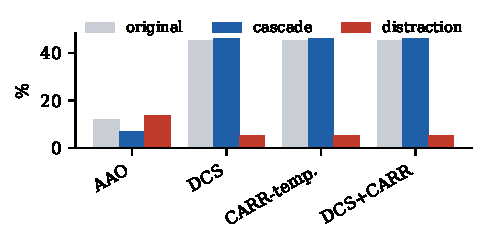
\includegraphics[width=0.95\columnwidth]{figures/cascade.pdf}
\caption{CARMA-Cascade (\texttt{ministral-14b}): step accuracy on original vs.\ cascaded logs, and distraction rate (share of predictions on the injected step).}
\label{fig:cascade}
\end{figure}

\textbf{Longer logs: the hand-crafted subset.} Table~\ref{tab:main_hand} reports 57 of the 58 hand-crafted logs (one log failed after retries with both methods). These logs average 51.6 steps, against 8.7 in the algorithm-generated subset, and both methods are close to the floor: All-at-Once reaches 3.5\% and DCS 5.3\% strict step accuracy (2 and 3 logs; McNemar $p=1.0$), comparable to the 5.3\% and 7.0\% reported for All-at-Once and Step-by-Step with GPT-4o~\cite{zhang2025whowhen}. The second judge's DCS reaches 3.5\%. The list again carries more information than its first entry: the gold step is among the top three DCS candidates in 19.3\% of logs with the main judge, against 3.5\% for the single step of All-at-Once, and anywhere in the list in 28.1\% (second judge: 33.3\%). DCS predicts a step before $t^*$ in 46 of 57 logs, so the earliness seen on the shorter logs is stronger here. Its agent accuracy (26.3\%, against 59.6\% for All-at-Once) is low by construction: DCS reads the agent from its predicted step, and on 21 of 58 hand-crafted logs the annotated agent is not the one speaking at the gold step (Section~\ref{sec:method}). With the second judge, All-at-Once and DCS are both correct on 2 of 57 logs (3.5\%, McNemar $p=1.0$), and All-at-Once names the right agent in 64.9\% of logs. Long logs remain essentially unsolved by single-call judges of this size, and we do not claim an improvement on them.

\IfFileExists{tables/main_hand.tex}{\begin{table*}[t]
\centering
\caption{Hand-crafted (Magentic-One) subset, logs within the API token budget ($n=6$).}
\label{tab:main_hand}
\footnotesize
\setlength{\tabcolsep}{4pt}
\begin{tabular}{@{}lcccccccccc@{}}
\toprule
Method & Agent & Step & 95\% CI & Acc@$\pm$1 & Top-3 & RTR & WRE$\downarrow$ & Calls & Tokens & $p$ vs AAO \\
\midrule
All-at-Once~\cite{zhang2025whowhen} & 83.3 & 0.0 & [0.0, 0.0] & 16.7 & 0.0 & 83.3 & 26.8 & 1.0 & 14.2k & -- \\
DCS top-1 (ours) & 16.7 & 0.0 & [0.0, 0.0] & 16.7 & 33.3 & 100.0 & 27.4 & 1.0 & 14.1k & 1.000 \\
\textbf{DCS + CARR (ours)} & 16.7 & 0.0 & [0.0, 0.0] & 16.7 & 16.7 & 100.0 & 27.4 & 1.0 & 14.1k & 1.000 \\
\bottomrule
\end{tabular}
\end{table*}}{}

\subsection{Ablation Studies and Additional Validation}\label{sec:ablation}
\textbf{Resolution ablation.} Table~\ref{tab:ablation} replaces the resolution step while keeping the same DCS candidates. Picking the earliest candidate, or the earliest candidate the judge itself tagged as an ``origin'', lowers step accuracy slightly (38.9\% each) and raises RTR, as expected from systematically earlier predictions; neither difference is significant ($p=0.73$ and $0.69$). Full CARR and CARR with a purely temporal graph give exactly the DCS top-1 result on every trajectory with the main judge, but CARR slightly lowers top-3 coverage (71.4\% to 70.6\% on algorithm-generated logs, 19.3\% to 15.8\% on hand-crafted logs). With the second backbone, CARR changes two predictions, both from correct to wrong (41.3\% to 39.7\%, $p=0.5$).

\begin{table*}[t]
\centering
\caption{Ablation of the resolution step on the same DCS candidates (algorithm-generated) ($n=126$).}
\label{tab:ablation}
\footnotesize
\begin{tabular}{@{}lcccccccccc@{}}
\toprule
Method & Agent & Step & 95\% CI & Acc@$\pm$1 & Top-3 & RTR & WRE$\downarrow$ & Calls & Tokens & $p$ vs CARR \\
\midrule
DCS top-1 (ours) & 57.1 & 40.5 & [31.7, 49.2] & 56.3 & 71.4 & 90.5 & 21.7 & 1.0 & 4.0k & 1.000 \\
DCS earliest cand. & 57.1 & 38.9 & [31.0, 47.6] & 55.6 & 67.5 & 93.7 & 23.4 & 1.0 & 4.0k & 0.727 \\
DCS earliest `origin' tag & 57.9 & 38.9 & [30.2, 46.8] & 56.3 & 71.4 & 92.9 & 23.0 & 1.0 & 4.0k & 0.688 \\
DCS + CARR, temporal graph & 57.1 & 40.5 & [31.7, 49.2] & 56.3 & 71.4 & 90.5 & 21.7 & 1.0 & 4.0k & 1.000 \\
\textbf{DCS + CARR (ours)} & 57.1 & 40.5 & [31.7, 49.2] & 56.3 & 70.6 & 90.5 & 21.7 & 1.0 & 4.0k & -- \\
\bottomrule
\end{tabular}
\end{table*}

\textbf{Why CARR does not change the ranking: over-confidence.} The judge returns on average 4.4 candidates, and its top candidate has a mean probability of 0.79 on original logs while being correct only 41\% of the time; the expected calibration error is 0.38 (0.30 on cascaded logs; 0.32 for the second judge). The probabilities are nevertheless informative as a ranking: the top candidate is correct in 82\% of logs when $p_1\ge0.9$ but in only 15--21\% when $p_1<0.8$ (Fig.~\ref{fig:offsets}). In Eq.~(\ref{eq:carr}), an earlier candidate $j$ discounts the top candidate by the factor $1-\gamma p_jP_{ji}\ge 1-p_j$, and the runner-up's explanation bonus is at most $1+\beta\sum_k p_k\approx1.5$ for $\beta=0.5$. Overturning a top probability that is typically five or more times the runner-up's (median ratio 5.7) would need both a near-certain earlier candidate and a strong provenance path, which almost never occurs. The provenance graph itself is informative (the gold step has an outgoing artifact edge in 61.1\% of algorithm-generated logs), and the room for a better re-ranker is large: top-1 is 40.5\% while the gold step is in the list 84.9\% of the time.

\textbf{Is sharpness the whole story?} In a post-hoc check (not pre-registered; \texttt{scripts/flatten\_carr.py}) we flattened the DCS probabilities, $p_k\propto p_k^{1/\tau}$ for $\tau\in\{2,3,5,10,\infty\}$, before applying CARR with the pre-registered $\gamma,\beta$. Flattening does let CARR change predictions (up to 13 of 126 with the 14B judge), but the changes cancel out: across both judges and both original and cascaded logs, no setting differs significantly from DCS top-1 (smallest $p=0.21$, a loss), and the direction of the change is not consistent across judges or log types. Over-confidence explains why CARR is inert at $\tau=1$, but once it can act, lexical provenance does not identify the root better than the judge's own ranking. Using the room between top-1 and top-5 coverage will need a stronger signal than shared artifacts, for example provenance given to the judge before it scores, or verification by re-execution as in~\cite{ma2025dover,rafi2026falat}.

\textbf{Sensitivity.} We swept $\gamma\in\{0,0.25,0.5,0.75,1\}$ and $\beta\in\{0,0.25,0.5,1,2\}$ (25 settings). With the main judge, step accuracy is identical in every setting (40.5\% original, 45.9\% cascade). With the second backbone it ranges from 39.7\% to 41.3\% on the original logs. The pre-registered values are not a tuned optimum, and no setting turns CARR into a significant improvement.

\textbf{Cost.} All methods compared in Table~\ref{tab:main_full} use one LLM call per trajectory and about 4k tokens; the APG and CARR run in a few milliseconds per trajectory on the CPU (below 3\,ms for the longest log, $T=130$). Binary Search uses 3.4 calls and 6.7k tokens per log on the 60-log sample, about 1.8 times the tokens of DCS.

\textbf{Summary of findings.} For O1, the reproduced baseline's step accuracy lies within the 95\% confidence interval of the published value and its agent accuracy within two points. Strict scoring changes step accuracy by 1.6 points on this subset, and the unnumbered protocol leaves the baseline unable to predict step~0. Most of the DCS gain with the stronger judge comes from numbering the log, so a protocol should fix numbering for every method. The further gain of the DCS prompt is partly a preference for early steps, and on logs with $t^*>0$ it survives only for the weaker judge. For O2, the DCS prompt is what keeps a judge on the decisive step when a later error is present. With the same judge and the same numbered log, All-at-Once is drawn to the injected step 2.3 to 8.5 times as often. The provenance re-ranking adds nothing to this, because the judge's probabilities are over-confident and, once flattened, lexical provenance does not rank better than the judge. For O3, DCS predictions are at or before the decisive step in nine of ten cases at no extra cost. This is an offline proxy, which the step-0 rule beats on coverage but not on discarded work, and the list works as a short rollback schedule.

\section{Conclusion and Future Work}\label{sec:concl}
We studied failure attribution in LLM multi-agent systems under one fixed evaluation protocol. Reproducing the All-at-Once judge of Who\&When with an open-weight backbone (\texttt{ministral-14b}) recovered the published agent and step accuracy on the algorithm-generated subset to within two points. It also showed that, on unnumbered logs, the judge cannot point at the first step at all, which is where 20 of 126 decisive errors are.

We proposed CARMA. Its DCS component asks the judge once for a scored list of candidate error steps over a numbered log, and its CARR component re-ranks that list with a deterministic artifact-provenance graph. We also built CARMA-Cascade, which adds one injected later error to each log, and measured how often a method is drawn to it. DCS raises strict step accuracy by 26--28 points over the official protocol with two judges at one call per log. Most of that gain, 16.7 points with the stronger judge, comes from numbering the log alone, and the candidate list helps ranking and rollback scheduling but not the first answer. The clearest benefit of the DCS prompt beyond numbering is resistance to distraction: on the same cascaded logs, numbered All-at-Once is drawn to the injected step 2.3 to 8.5 times as often as DCS. CARR did not improve on DCS, because the judge's probabilities are strongly over-confident, and we report this negative result with its cause.

The study has clear limits. No method improves on the long hand-crafted logs, where everything is near the floor. Both judges come from one provider, each condition was run once despite measurable run-to-run variability, the cascade errors are synthetic and independent of the original error, Binary Search was evaluated only on a 60-log sample, and Step-by-Step was not run. Three directions follow. The first is to calibrate the DCS probabilities, or give provenance to the judge before it scores, so that structural evidence can change the ranking. The second is to evaluate on longer traces with naturally occurring multiple errors and stronger judges, with several runs per condition. The third is to test the candidate list as a rollback schedule in a system that can re-execute runs, turning the offline proxy into measured recovery.

\bibliographystyle{IEEEtran}
\bibliography{refs}

\end{document}
